\documentclass[12pt]{article}
\setlength\parindent{0pt}
\usepackage{fullpage}
\usepackage{amsmath}
\usepackage{graphicx}
\setlength{\parskip}{4mm}
\def\LL{\left\langle}   % left angle bracket
\def\RR{\right\rangle}  % right angle bracket
\def\LP{\left(}         % left parenthesis
\def\RP{\right)}        % right parenthesis
\def\LB{\left\{}        % left curly bracket
\def\RB{\right\}}       % right curly bracket
\def\PAR#1#2{ {{\partial #1}\over{\partial #2}} }
\def\PARTWO#1#2{ {{\partial^2 #1}\over{\partial #2}^2} }
\def\PARTWOMIX#1#2#3{ {{\partial^2 #1}\over{\partial #2 \partial #3}} }
\newcommand{\BE}{\begin{displaymath}}
\newcommand{\EE}{\end{displaymath}}
\newcommand{\BNE}{\begin{equation}}
\newcommand{\ENE}{\end{equation}}
\newcommand{\BEA}{\begin{eqnarray}}
\newcommand{\EEA}{\nonumber\end{eqnarray}}
\newcommand{\EL}{\nonumber\\}
\newcommand{\la}[1]{\label{#1}}
\newcommand{\ie}{{\em i.e.\ }}
\newcommand{\eg}{{\em e.\,g.\ }}
\newcommand{\cf}{cf.\ }
\newcommand{\etc}{etc.\ }
\newcommand{\Tr}{{\rm tr}}
\newcommand{\etal}{{\it et al.}}
\newcommand{\OL}[1]{\overline{#1}\ } % overline
\newcommand{\OLL}[1]{\overline{\overline{#1}}\ } % double overline
\newcommand{\OON}{\frac{1}{N}} % "one over N"
\newcommand{\OOX}[1]{\frac{1}{#1}} % "one over X"



\begin{document}
\Large
\centerline{\sc{Homework 4}}
\normalsize
\centerline{\sc{Due Friday, 24 February}}

{\sc Note:} For all problems, in order to receive credit, you must draw force diagrams for all relevant objects. These diagrams must be at least two inches tall to receive full credit.
This is for your benefit, not mine; carefully drawing clear diagrams will help you with these problems more than anything else.

\begin{enumerate}


  \begin{minipage}{0.7\textwidth}
\item  An object of mass $M$ sits on a frictionless table; it is connected by
   a light string to a hanging mass $m$. (See figure.)
\begin{enumerate}
\item Find an expression for the tension in the string in terms of $M$, $m$, and $g$.
\item Find the acceleration of the masses in terms of $M$, $m$, and $g$.
\item What is the tension in the limit where $M \gg m$ (that is, the mass on the table is very heavy)? Is this what you expect it to be?
\item What is the acceleration in the limit where $m \gg M$ (that is, the hanging mass is very heavy)? Is this what you expect it to be?
\end{enumerate}
  \end{minipage}
  \begin{minipage}{0.3\textwidth}
\centerline{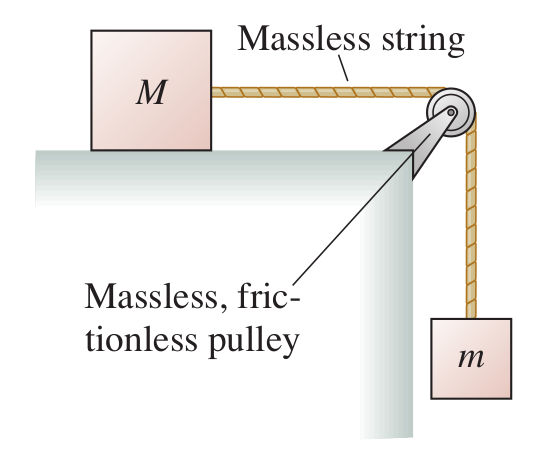
\includegraphics[width=0.9\textwidth]{problem736.png}}
  \end{minipage}

\bigskip

  \begin{minipage}{0.7\textwidth}
\item Two masses are connected by a light string and draped over a light, frictionless pulley. One has mass $m$, which you will find; the other has mass $M=100$ kg. (See figure.)
   
\begin{enumerate}
\item Find an expression for the acceleration of the mass $M$ in terms of $M$, $m$,
and $g$.
\item If it takes a time $\tau=6$ s to hit the ground after it is released, what is
the value of $m$? 
\end{enumerate}
  \end{minipage}
  \begin{minipage}{0.3\textwidth}
\centerline{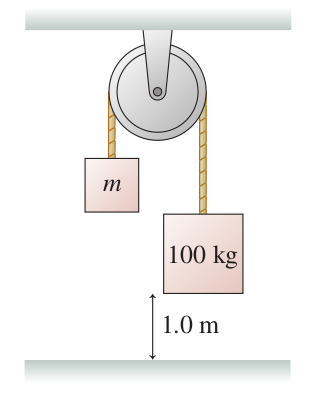
\includegraphics[width=0.9\textwidth]{problem738.png}}
  \end{minipage}


\bigskip

  \begin{minipage}{0.6\textwidth}
\item A rope-and-pulley system is set up as shown. What is the acceleration of the 
2 kg block sitting on the table? 
   
the value of $m$? 
  \end{minipage}
  \begin{minipage}{0.4\textwidth}
\centerline{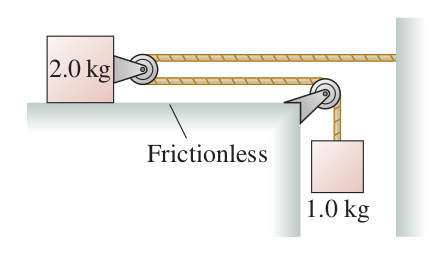
\includegraphics[width=0.9\textwidth]{problem755.png}}
  \end{minipage}

Hint: Think very carefully about how the acceleration of the two blocks relates.
If the hanging mass moves downward by one meter, how far does the block on the table
move?



\bigskip


  \item{A block of mass $m_1=5$ kg rests on a table. Two ropes connect that block to two masses that hang off the sides of the table. The coefficient of static friction $\mu_s$ between the block and the table is 0.2.\\
    
    If one of the hanging masses has mass $m_2=3$ kg, for what range of values of the other block's mass $m_3$ will the system not move?\\
  
  {\sc Hint 1}: What happens if $m_3$ is very small? What happens if it is very big? Does this affect your force diagram in any way? How do you know what direction
static friction will point? Does this depend on the sizes of the masses?
{\sc Hint 2}: If you use the same variable $a$ for acceleration in all your equations, make sure that it has the same value for all the objects! This may require careful choice of your coordinate axes.}


\bigskip

\item{Two blocks slide down an incline angled at $20^\circ$ above the horizontal, connected by a cable. The top block has a mass of $m_1=1$ kg, and the bottom one has a mass of $m_2=2$ kg. The coefficients of kinetic friction are 
  $\mu_{k_1}=0.2$ (top block) and $\mu_{k_2}=0.1$ (bottom block). What is the tension in the cable that connects them?}


\bigskip

\item{A hiker with a mass of 75 kg wants to drag a 200 kg sled over snow. She does this by tying a rope to the sled (at ground level) and running it over her shoulder. The rope running between her and the sled makes a 45 degree angle with the horizontal.

  If the coefficient of friction between the sled and the snow is 0.1, what must the coefficient of friction between her boots and the ground be for her to move the sled?}


    \end{enumerate}
\end{document}
